\documentclass{beamer}

\usepackage[utf8]{inputenc}
\usepackage{booktabs}
\usepackage{xcolor}
%\usetheme{Hannover}
\usecolortheme{crane}
\usepackage{siunitx,cancel}
\usepackage{graphicx}
\usepackage{hyperref}

\usepackage{listings}
\usepackage{color}
\usepackage{xcolor}

%\usepackage[
%backend=biber,
%style=numeric,
%citestyle=numeric,
%sorting=none
%]{biblatex}
%\addbibresource{resources.bib}


% This is the color used for MATLAB comments below
\definecolor{MyDarkGreen}{rgb}{0.0,0.4,0.0}
\definecolor{Blue}{rgb}{0.0,0.0,1.0}
\definecolor{Purple}{rgb}{1.0,0.0,1.0}

\colorlet{mygray}{black!30}
\colorlet{mygreen}{green!60!blue}
\colorlet{mymauve}{red!60!blue}

\lstset{
  backgroundcolor=\color{gray!10},
  basicstyle=\ttfamily,
  columns=fullflexible,
  breakatwhitespace=false,
  breaklines=true,
  captionpos=b,
  commentstyle=\color{mygreen},
  extendedchars=true,
  frame=single,
  keepspaces=true,
  keywordstyle=\color{blue},
  language=c++,
  numbers=none,
  numbersep=5pt,
  numberstyle=\tiny\color{blue},
  rulecolor=\color{mygray},
  showspaces=false,
  showtabs=false,
  stepnumber=5,
  stringstyle=\color{mymauve},
  tabsize=3,
  title=\lstname
}






%\defaultfontfeatures{Scale=MatchLowercase,Mapping=tex-text}
%\setmainfont[Numbers=Lowercase]{Minion Pro}
%\setsansfont[Numbers=Lowercase]{Myriad Pro}
%\setmonofont{Menlo}
%\setmathsfont(Digits,Latin,Greek)[Numbers={Lining,Proportional}]{Minion Pro}

\sisetup{%
  output-decimal-marker = {.},
  per-mode = symbol,
  %round-mode = places,
  %round-precision = 5
}

\DeclareSIUnit \electronvolt {\ensuremath{eV}}
\DeclareSIUnit \lightspeed {\ensuremath{c}}
\DeclareSIUnit \dalton{\ensuremath{u}}
\DeclareSIUnit \echarge{\ensuremath{e}}


\newcommand{\mvec}[2]{
\ensuremath{\left(
\begin{array}{c}
#1\\
#2\\
\end{array}
\right)}
}

\newcommand{\Span}{\ensuremath{\mathrm{Span}}}
\newcommand{\Mat}{\ensuremath{\mathrm{Mat}}}
\newcommand{\R}{\ensuremath{\mathbb{R}}}
\newcommand{\Rno}{\ensuremath{\mathbb{R}\backslash\{0\}}}
\newcommand{\Z}{\ensuremath{\mathbb{Z}}}
\newcommand{\ol}[1]{\ensuremath{\overline{#1} } }
\newcommand{\F}[1]{\ensuremath{\mathbb{F}_{#1} } }

\newif\ifdraft

\drafttrue
\draftfalse

%Information to be included in the title page:
\title{How physics simulations work: simulating particles in electric and magnetic fields}
%Numerical integration of ordinary differential equations: motion of charged particles in electromagnetic fields}
\author{Nikolaj Roager Christensen}
\institute{Student Colloquium in Physics and Astronomy, Aarhus University}
\date{May 2022 CE}

%\AtBeginSection[]
%{
%ect

%\titlegraphic
%{
%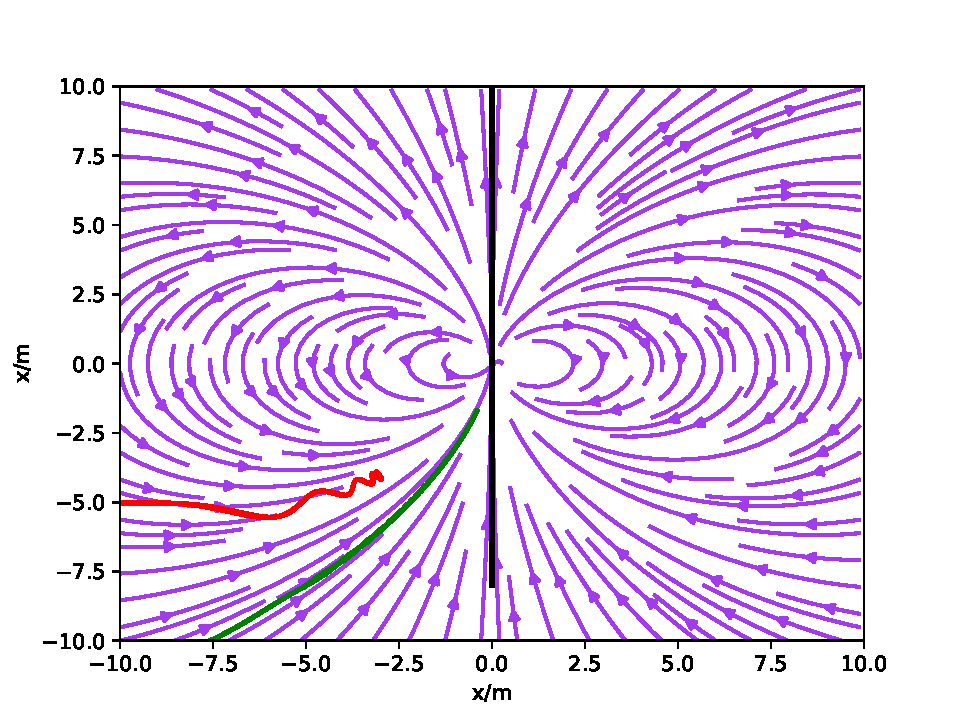
\includegraphics[width=0.5\textwidth]{dipole6.pdf}
%}
\begin{document}

{
\setbeamertemplate{background}
{
    \centering
    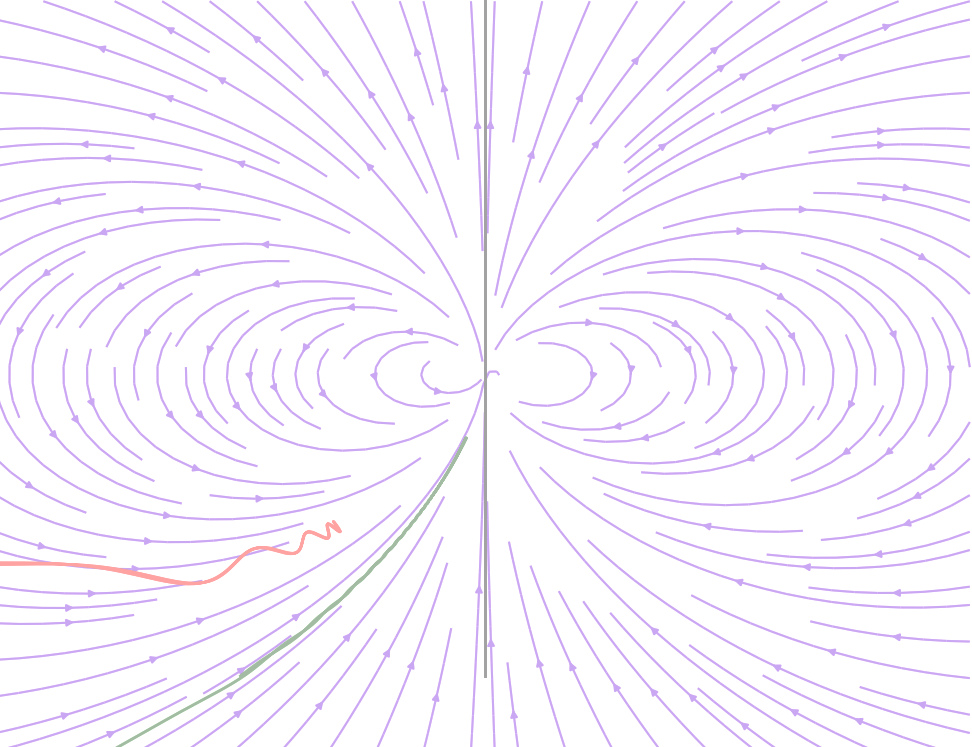
\includegraphics[width=\paperwidth]{dipole_preface.png}
}
\frame{\titlepage}
}


\section{Introduction}

\begin{frame}
\frametitle{How physics simulations work: simulating particles in electric and magnetic fields.}
\tableofcontents
\end{frame}


\begin{frame}
\frametitle{Motivation and introductions.}
\begin{itemize}
\item<1-> Numerical simulations are important.
\item<2-> Testing setups, non-analytical systems.
\item<3-> Engineering: testing integrity of buildings/machines.
\item<4-> Entertainment: Video-games and CGI effects in movies.
\item<5-> Demonstration, charged particles in electric and magnetic fields.
\item<6-> Simulations are not experiments!
\end{itemize}
\end{frame}

\ifdraft
    \section{Theory and physical background 10 min}
\else
    \section{Theory and physical background}
\fi

\begin{frame}
\frametitle{Theory: Classical non-relativistic particles.}
\begin{itemize}
\item<1-> Some repetition from Electrodynamics.
\item<2-> The Lorentz force+N2:

\begin{align*}
\vec{F} &= q ( \vec{v}\times \vec{B}+\vec{E}).\\
\ddot{\vec{r}}(t) &= \frac{q}{m} ( \dot{\vec{r}}(t)\times \vec{B}(\vec{r},t)+\vec{E}(\vec{r},t)).
\end{align*}

\item<3-> Could use potentials $\phi(\vec{r},t)$ $\vec{A}(\vec{r},t)$ and Hamiltonian, or Lagrangian.

\item<4-> Other systems would have other differential equations.

\end{itemize}
\end{frame}


\begin{frame}
\frametitle{Known results, cyclotron motion $\vec{B}$ fields.}
\begin{columns}
\begin{column}{0.5\linewidth}
\begin{itemize}
\item<2-> Magnetic forces do no work:

\begin{equation*}
dW_{\vec{B}}= \vec{F}_B \cdot d\vec{r}\propto (\vec{v}\times \vec{B})\cdot \vec{v} = 0.
\end{equation*}

\item<3-> ($\vec{v}=\vec{v}_\perp+\vec{v}_\parallel$):

\begin{equation*}
|\vec{F}_B| = |q ( \vec{v}\times \vec{B})| =|q v_{\perp} B|.
\end{equation*}
\item<4-> Same as Centripetal force: Cyclotron motion.

\item<5-> Cyclotron radius and frequency:

\begin{equation*}
R = \frac{v_\perp m}{|q|B} \quad \omega_c =\frac{|q|B}{m}.
\end{equation*}

\end{itemize}
\end{column}
\begin{column}{0.5\linewidth}
\only<1-2>{%
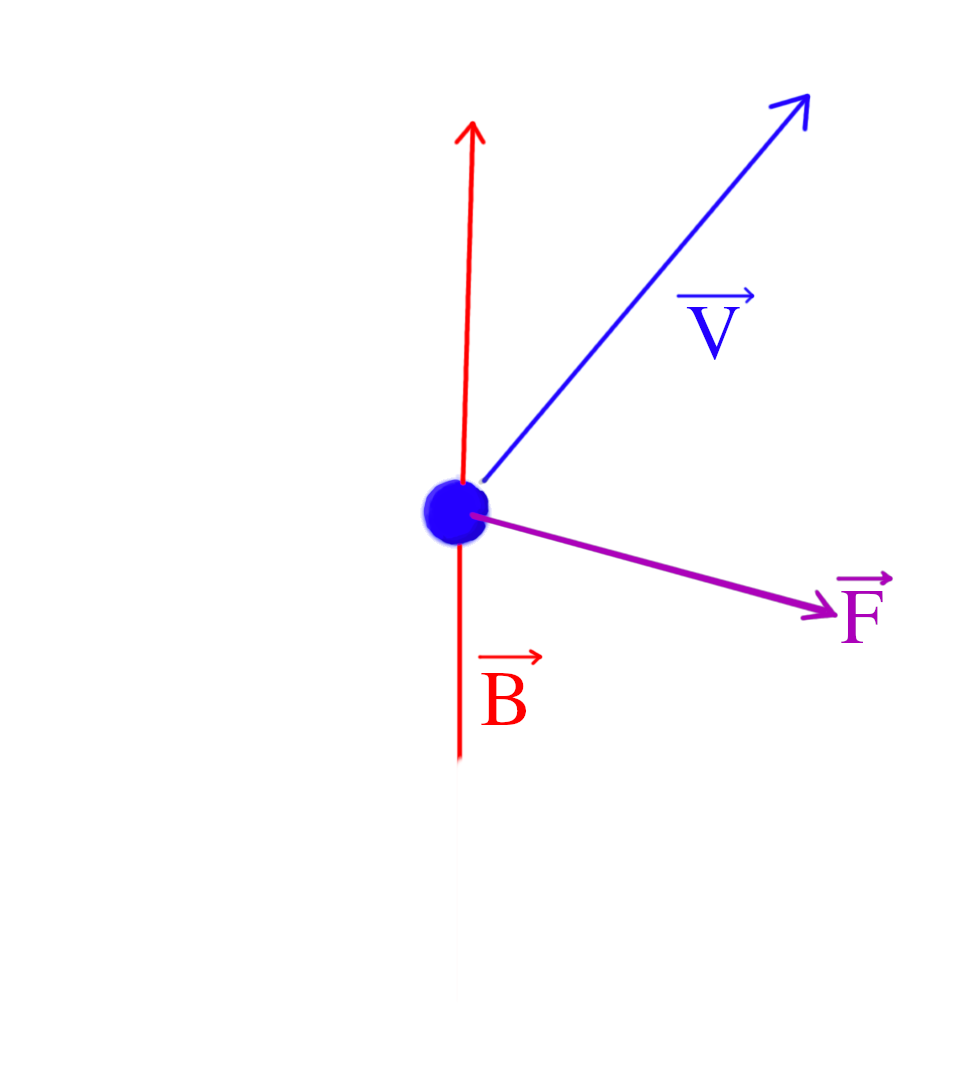
\includegraphics[width=\linewidth]{dw0.png}}%
\only<3->{%
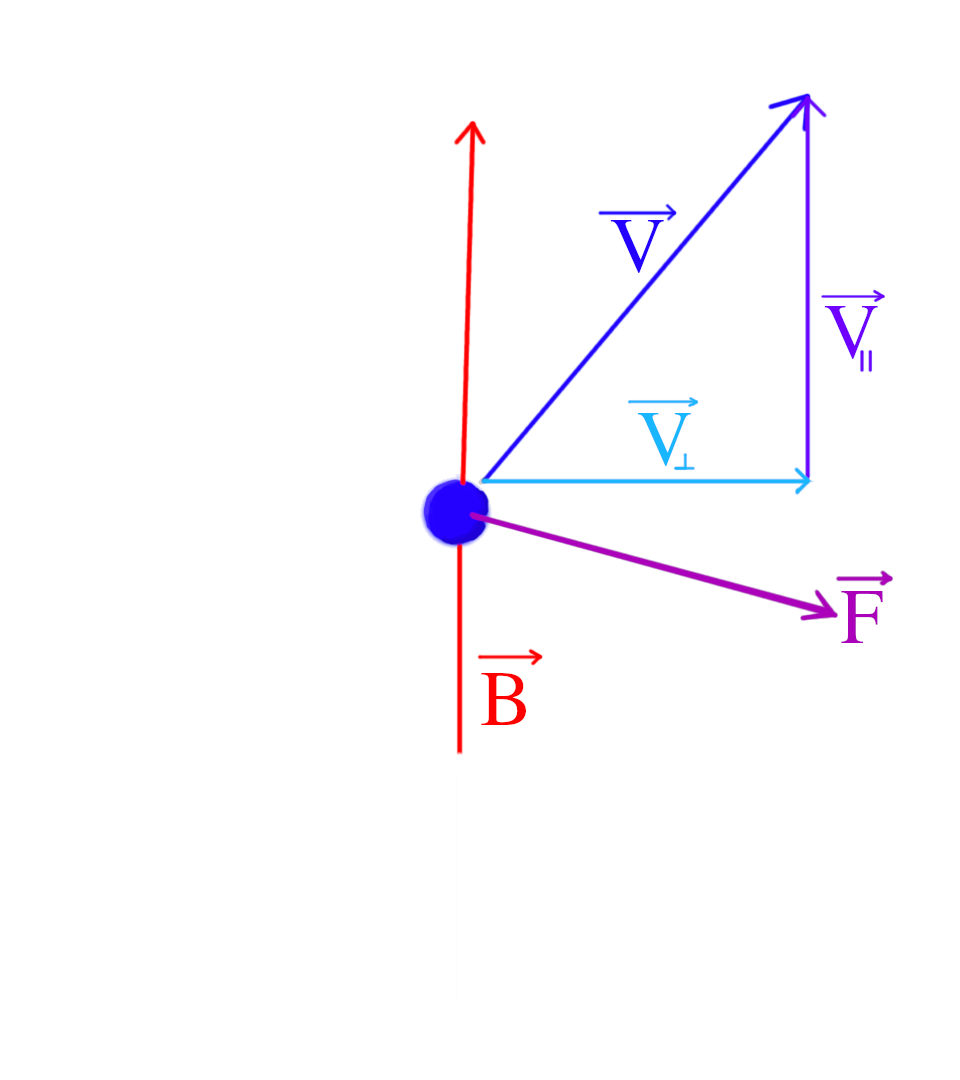
\includegraphics[width=\linewidth]{cyc0.png}}%
%\only<4->{%
%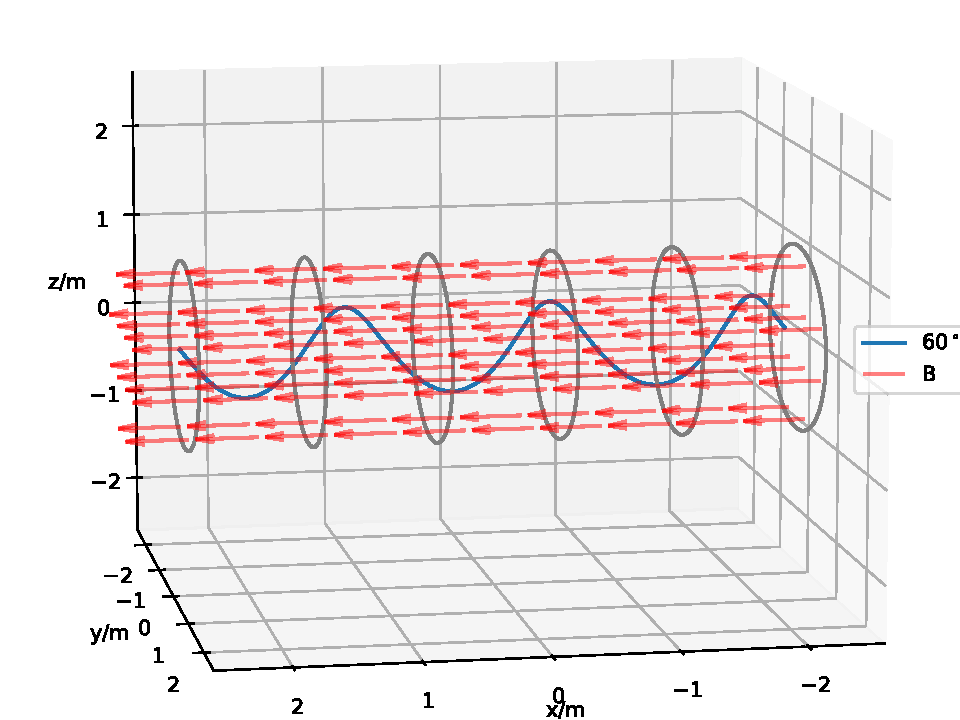
\includegraphics[width=\linewidth]{helix.pdf}}%
\end{column}
\end{columns}
\end{frame}

\begin{frame}
\frametitle{What we expect to see.}
\only<1>{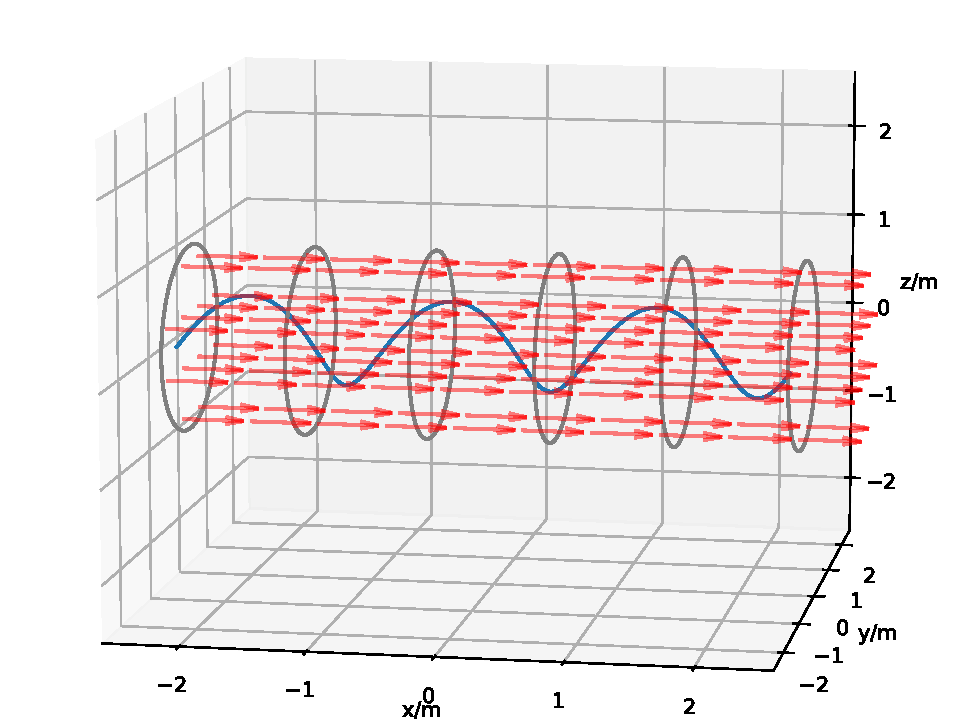
\includegraphics[width=0.8\linewidth]{AN_helix0.pdf}}%
\only<2>{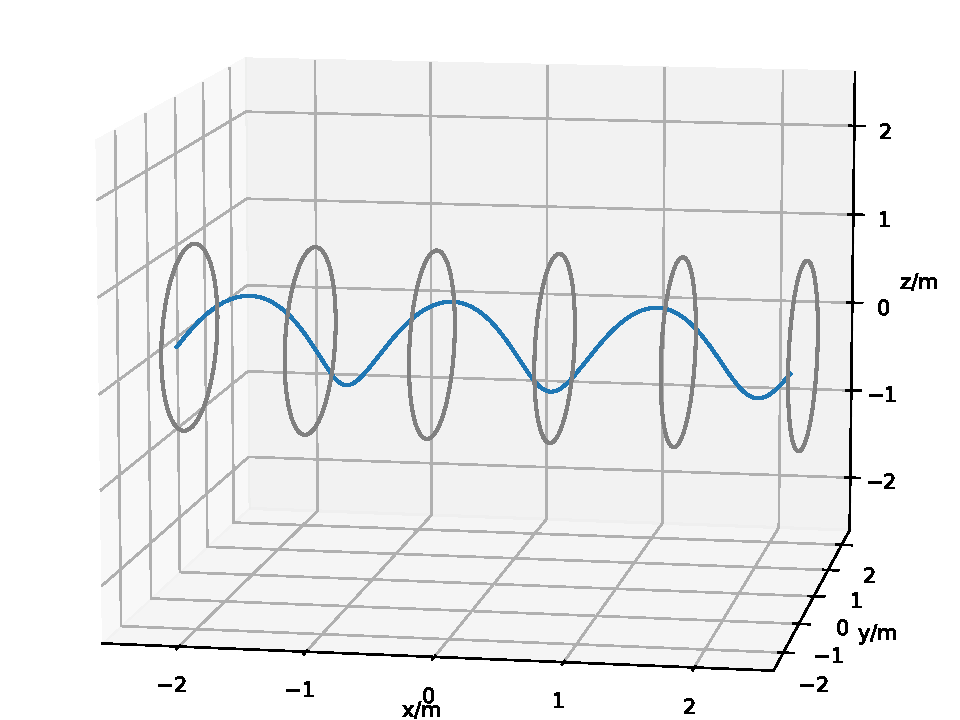
\includegraphics[width=0.8\linewidth]{AN_helix1.pdf}}%
\only<3>{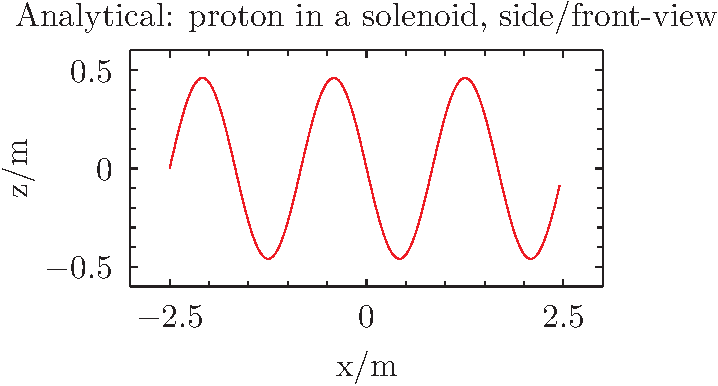
\includegraphics[width=0.66\linewidth]{AN_solenoid_xz_view.pdf}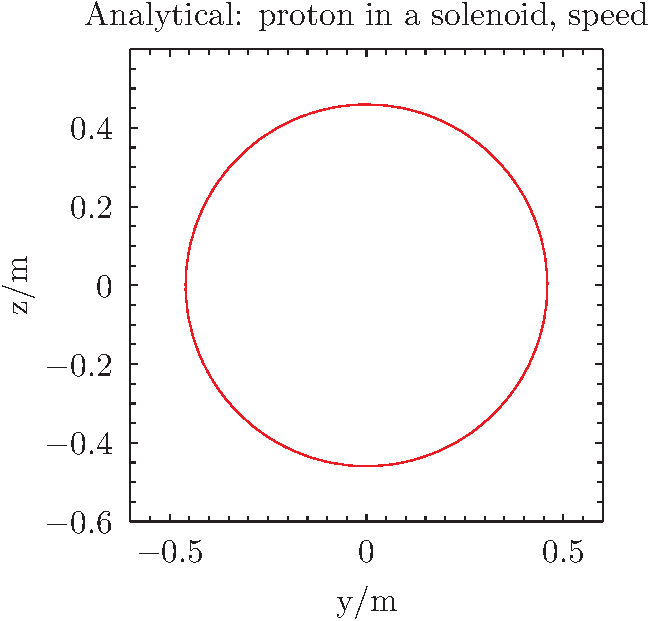
\includegraphics[width=0.33\linewidth]{AN_solenoid_yz_view.pdf}}%
\only<4>{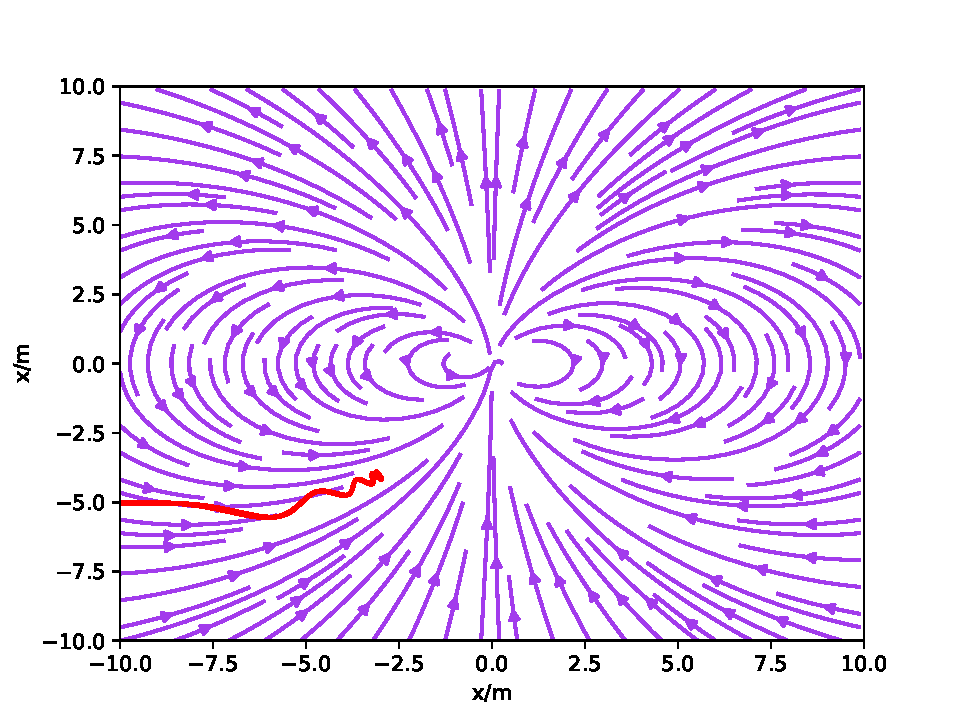
\includegraphics[width=0.8\linewidth]{dipole7.pdf}

(Actually from my simulation)}%

\only<1>{%
``Cyclotron motion"

{\color{gray} Solenoid with $N=1000$ turns per $m$, $I=\SI{5}{\ampere}$, $r=\SI{1}{\meter}$, $|\vec{B}|\approx\SI{6}{\milli\tesla}$. Proton with $|v|\approx \SI{3.195E5}{\meter\per\second}$}}

\only<2-3>{%
``Cyclotron motion"

\begin{equation*}
R \approx \SI{0.5}{\meter}\sin(\theta) \quad T_c=\frac{2\pi}{\omega_c} \approx \SI{10}{\micro\second}
\end{equation*}
}
\end{frame}

\ifdraft
    \section{Euler's Method and the 4th order Runge-Kutta Method 15 min}
\else
    \section{Euler's Method and the 4th order Runge-Kutta Method}
\fi
%What are they, what are not they

\begin{frame}
\frametitle{Ordinary differential equation's.}
\begin{itemize}
\item<1-> {\color{gray} Sources: Zeigler et al. Theory of Modeling and Simulation (Third edition) chapter 3}.

\item<1-> We have:

\begin{align*}
\ddot{\vec{r}}(t) &= \frac{q}{m} ( \dot{\vec{r}}(t)\times \vec{B}(\vec{r},t)+\vec{E}(\vec{r},t)).
\end{align*}

\item<2-> Algorithms exists for ODEs:

\begin{equation*}
\dot{\mathbf{X}} = \mathbf{f}_{ode}(\mathbf{X}(t),t).
\end{equation*}


\item<3-> Here:

\begin{align*}
\mathbf{X} = \mvec{\vec{r}}{\dot{\vec{r}}} \quad \mathbf{f}_{ode}(\mathbf{X},t) = \mvec{\dot{\vec{r}}}{\frac{q}{m} ( \dot{\vec{r}}\times \vec{B}(\vec{r},t)+\vec{E}(\vec{r},t))}.
\end{align*}
\end{itemize}
\end{frame}

%\begin{frame}[fragile]
%\frametitle{The ODE to solve}
%\only<1>{%
%\begin{lstlisting}
%auto ODE = [...](const state_type Data, state_type &dDatadt, const double t){
%    //Extract position and velocity from data
%    vec pos = vec(Data[0],Data[1],Data[2]);
%    vec V = vec(Data[3],Data[4],Data[5]);
%    //Lorentz+Newtons 2nd law
%    vec F = Charge*(Fields.get_Efield(pos,t)+
%        cross(V,Fields.get_Bfield(pos,t)));
%    vec dVdt = F*Inv_mass;
%    //Save derivative of data
%    dDatadt[0]=V.x;dDatadt[1]=V.y;dDatadt[2]=V.z;
%    dDatadt[3]=dVdt.x;Datadt[4]=dVdt.y;dDatadt[5]=dVdt.z;
%    };
%\end{lstlisting}
%\end{frame}


\subsection{Euler's Method}

\begin{frame}
\frametitle{Solving differential equations.}
\begin{itemize}

\item<1-> We know only $\mathbf{X}(t_i)$ and $t_i= t_0+i \Delta t$ and $\mathbf{f}_{ode}$.

\item<2-> Can we find $\mathbf{X}(t_i+\Delta t)$ for $\Delta t>0$?

\item<3-> Euler's Method:

\begin{equation*}
\mathbf{X}(t_i+\Delta t) = \mathbf{X}(t_i)+\Delta t \mathbf{f}_{ode}(\mathbf{X}(t_i),t_i).
\end{equation*}

\item<3-> Multiple steps $t_0,t_1=t_0+\Delta t,\ldots t_i,\ldots$.

\item<4-> Can this be justified?

\item<1-> {\color{gray} Bernard P. Zeigler et al. Theory of Modeling and Simulation (Third edition), chapter 3.}
\end{itemize}
\end{frame}


\begin{frame}
\frametitle{Why does this work? What is the error.}
\begin{itemize}
\item<1-> Multiple justifications for why.

\item<2-> First 2 terms in Taylor series {{\color{gray} Zeigler et al.}}:

\begin{equation*}
\only<1>{\mathbf{X}(t_{i}+\Delta t) = \mathbf{X}(t_{i})+\Delta t \dot{\mathbf{X}}(t_i)+\Delta t^2\ldots +\ldots}
\only<2->{\mathbf{X}(t_{i}+\Delta t) = \mathbf{X}(t_{i})+\Delta t \mathbf{f}_{ode}(\mathbf{X}(t_i),t_i)+\Delta t^2\ldots +\ldots}
\end{equation*}

\item<3-> Local error  $O((\Delta t)^{2})$.

\item<4-> We want ``better" (larger $\Delta t$  (fewer steps, fewer calls), same error).

\item<5-> Argument suggests we need $\dot{\mathbf{f}}_{ode},\ddot{\mathbf{f}}_{ode},\ldots$, we don't!
\end{itemize}
\end{frame}

\begin{frame}
\frametitle{The Runge Kutta steppers.}
\begin{itemize}

\item<1-> In general:

\begin{equation*}
\mathbf{X}(t_{i+1})-\mathbf{X}(t_{i}) \only<1->{=\int_{t_i}^{t_{i+1}}} \only<1>{\dot{\mathbf{X}}(t) dt}\only<2->{\mathbf{f}_{ode}(\mathbf{X}(t),t) dt }\only<3->{ = \Delta t \mathbf{f}_{ode}(\mathbf{X}(\tau),\tau)}.
\end{equation*}

\item <3-> \textit{Mean Value theorem for integrals} $t_i\leq \tau\leq t_{i+1}$.


\item<4-> More generally, (\textit{Explicit} and \textit{single step}), Runge-Kutta family:

\begin{align*}
\mathbf{X}(t_{i+1})-\mathbf{X}(t_{i}) &= \int_{t_i}^{t'} \mathbf{f}_{ode}(\mathbf{X}(t),t) dt + \ldots \int_{t^{(m)}}^{t_{i+1}} \mathbf{f}_{ode}(\mathbf{X}(t),t) dt \only<5->{,\\ &=  \sum_{j=1}^{m} \Delta t_j \mathbf{f}_{ode}(\mathbf{X}(\tau_j),\tau_j)}.
\end{align*}

\item<6-> Cant guess anything ... unless $\mathbf{X}(t)$ is polynomial.


\item<1-> {\color{gray} L. Zheng, X. Zhang, Modeling and Analysis of Modern Fluid Problems, 2017, chapter 8}:

\end{itemize}
\end{frame}


\begin{frame}
\frametitle{Runge Kutta methods.}
\begin{itemize}

\item<1-> More commonly written:

\begin{equation*}
\mathbf{X}(t_{i+1})-\mathbf{X}(t_{i}) =  \Delta t \sum_{j=1}^{m} b_j \mathbf{K}_j
\end{equation*}

\item<2-> Pick $\mathbf{K}_j$ so and pick an $m$:

\begin{align*}
\mathbf{K}_1 &= \mathbf{f}_{ode}(\mathbf{X}(t_i),t_i)\\
\mathbf{K}_2 &= \mathbf{f}_{ode}(\mathbf{X}(t_i)+\Delta ta_{21} \mathbf{K}_1,t_i+c_2 \Delta t)\\
\mathbf{K}_3 &= \mathbf{f}_{ode}(\mathbf{X}(t_i)+\Delta ta_{31} \mathbf{K}_1+\Delta ta_{32} \mathbf{K}_2,t_i+c_3 \Delta t)\\
&\vdots
\end{align*}

\item<3-> Pick parameters to be \textit{exact} for $p$'th order polynomial.

\item<4-> Taylor series analogy: Local error  $O((\Delta t)^{p+1})$.

\item<1-> {{\color{gray} Martha L. Abell, James P. Braselton, Differential Equations with Mathematica (Fourth Edition), 2016}}.
\end{itemize}
\end{frame}


\begin{frame}
\frametitle{The General explicit Runge Kutta method.}
\begin{itemize}


\item<1-> Expressed in Butcher tableu:

\begin{tabular}{l | @{\quad} c @{\quad} c @{\quad} c}
$c_1=0$ \\
$c_2$ & $a_{21}$\\
$c_3$ & $a_{31}$ &  $a_{32}$\\
$c_n$ & $a_{n1}$ &  $a_{n2}$ & $\hdots$\\
\midrule
& $b_1$ & $b_2$ & $\hdots$
\end{tabular}
\end{itemize}
\end{frame}

\subsection{Higher order Runge-Kutta methods}


\begin{frame}
\frametitle{Higher order methods.}
\begin{itemize}

\item<1-> 2nd order (Heun's method):

\begin{align*}
\mathbf{X}(t_{i+1})-\mathbf{X}(t_{i}) &= \frac{\Delta t}{2}(\mathbf{K}_1+\mathbf{K}_2),\\
\mathbf{K}_1 &= \mathbf{f}_{ode}(\mathbf{X}(t_i),t_i),\\
\mathbf{K}_2 &= \mathbf{f}_{ode}(\mathbf{X}(t_i)+\Delta t\mathbf{K}_1,t_i+\Delta t).
\end{align*}

\end{itemize}
\end{frame}

\begin{frame}
\frametitle{Higher order methods.}
\begin{columns}
\begin{column}{0.5\linewidth}
\begin{itemize}
\item<1-> 4th order, often simply called the Runge Kutta method:

\begin{align*}
\mathbf{X}(t_{i+1})-\mathbf{X}(t_{i}) &= \frac{\Delta t}{6}(\mathbf{K}_1+2\mathbf{K}_2+2\mathbf{K}_3+\mathbf{K}_4 )\\
\mathbf{K}_1 &= \mathbf{f}_{ode}(\mathbf{X}(t_i),t_i)\\
\mathbf{K}_2 &= \mathbf{f}_{ode}(\mathbf{X}(t_i)+\frac{\Delta t}{2}\mathbf{K}_1,t_i+\frac{\Delta t}{2})\\
\mathbf{K}_3 &= \mathbf{f}_{ode}(\mathbf{X}(t_i)+\frac{\Delta t}{2}\mathbf{K}_2,t_i+\frac{\Delta t}{2})\\
\mathbf{K}_4 &= \mathbf{f}_{ode}(\mathbf{X}(t_i)+\Delta t\mathbf{K}_3,t_i+\Delta t).
\end{align*}

\end{itemize}
\end{column}
\begin{column}{0.5\linewidth}
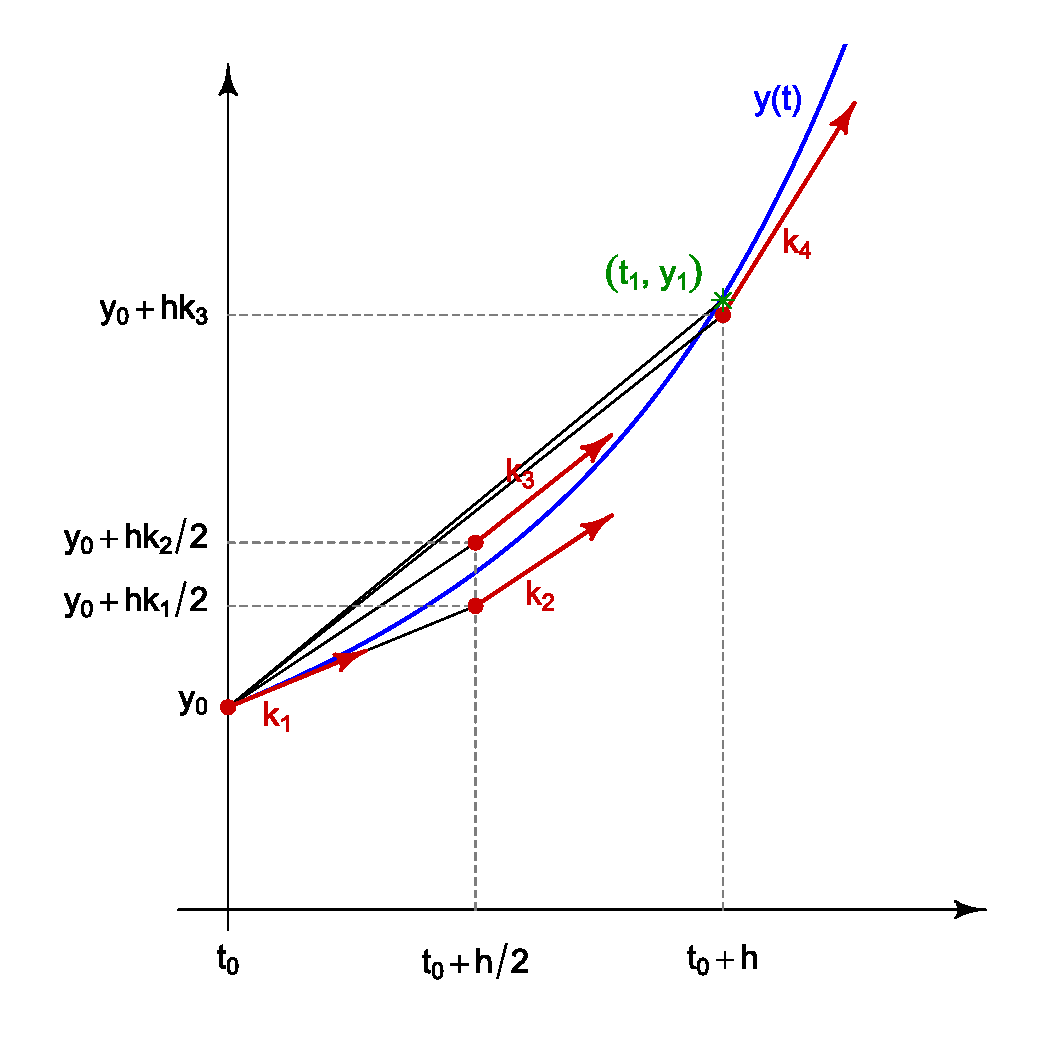
\includegraphics[width=\linewidth]{Runge-Kutta_slopes.pdf}

{\color{gray} Wikipedia-user HilberTraum, published under creative commins: CC BY-SA 4.0}
\end{column}
\end{columns}
\end{frame}

\ifdraft
\begin{frame}[fragile]
\frametitle{Euler Implementations}
\begin{lstlisting}
state_type Data = Data0;
state_type dDatadt;
size_t time_res = T/timestep;
for (size_t i = 1; i < time_res; ++i)
{
    double t=i*dt;
    ODE(Data,dDatadt,t);
    //Euler time evolution
    Data+=timestep*dDatadt;

    save_step( Data , i*timestep );
};
\end{lstlisting}
\end{frame}

\begin{frame}[fragile]
\frametitle{RK4 Implementations (1/2)}
\begin{lstlisting}
state_type Data = Data0;
state_type temp=Data0;
state_type K1,K2,K3,K4;
size_t time_res = T/timestep;
for (size_t i = 1; i < time_res; ++i)
{
    double t=i*timestep;

    //substep 1
    ODE(Data,K1,t);

    //substep 2
    temp=Data+timestep*K1/2;
    ODE(temp,K2,t+timestep/2);
\end{lstlisting}
\end{frame}

\begin{frame}[fragile]
\frametitle{RK4 Implementations (2/2)}
\begin{lstlisting}

    //substep 3
    temp=Data+timestep*K2/2;
    ODE(temp,K3,t+timestep/2);

    //substep 4
    temp=Data+timestep*K3;
    ODE(temp,K4,t+timestep);

    //Read data
    Data+=timestep*(K1+2.0*K2+2.0*K3+K4)/6.0;
    save_step( Data , i*timestep );}
}
\end{lstlisting}
\end{frame}
\fi

%\begin{frame}[fragile]
%\frametitle{``Correct" way}
%\begin{lstlisting}
%#include <boost/array.hpp>
%#include <boost/numeric/odeint.hpp>
%using namespace boost::numeric::odeint;
%typedef boost::array< double, 6 > state_type;
%...
%size_t steps = integrate_const(
%    runge_kutta4< state_type >(),
%    ODE,   //Lorentz-force
%    Data0 ,//{pos0,v0}
%    0.0 ,  //t0=0
%    T ,    //max time
%    timestep ,//length of each step
%    save_step //User defined save data function
%);
%\end{lstlisting}
%\end{frame}

\subsection{Demonstration, particles in a solenoid}

\begin{frame}
\frametitle{Does it work.}
\begin{itemize}

\item<1-> Test, same proton in a solenoid use same starting conditions with:

\begin{equation*}
R \approx  \SI{0.45}{\meter} \quad T_c=\frac{2\pi}{\omega_c} \approx \SI{10}{\micro\second}.
\end{equation*}

\item<2-> Compare Analytic, Euler, Runge-Kutta 4. At different $\Delta t_{equiv}$.

\item<3-> $\Delta t_{equiv}=4\Delta t$ for 4th order method.

\item<4-> Check error on $|\vec{v}|$, $R=\sqrt{y^2+z^2}$.

\end{itemize}
\end{frame}


\makeatletter
\begin{frame}
\frametitle{At a glance, 3D view.}
    \global\beamer@shrinktrue
    \gdef\beamer@shrinkframebox{
        \setbox\beamer@framebox=\vbox to\beamer@frametextheight{
            \centering
            $\Delta t_{equiv}\approx 1/1000 T_c$

            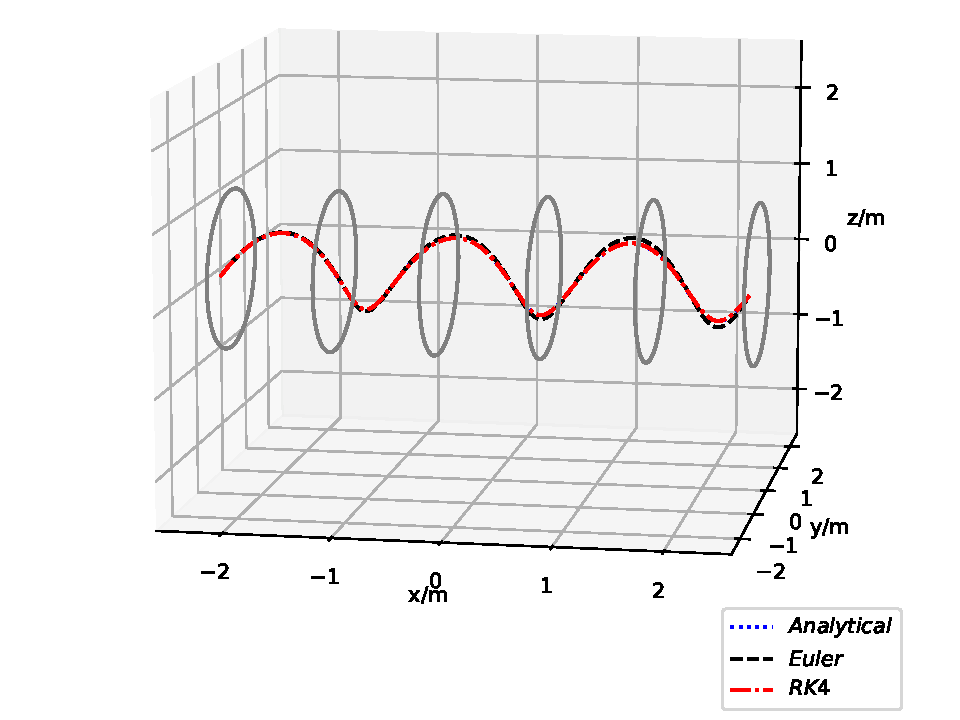
\includegraphics[height=0.9\beamer@frametextheight]{Solenoid_compare001_3D.pdf}

            3129 steps
        }
    }
\end{frame}
\makeatother

\makeatletter
\begin{frame}
\frametitle{At a glance, 3D view.}
    \global\beamer@shrinktrue
    \gdef\beamer@shrinkframebox{
        \setbox\beamer@framebox=\vbox to\beamer@frametextheight{
            \centering
            $\Delta t_{equiv}\approx 1/100 T_c$

            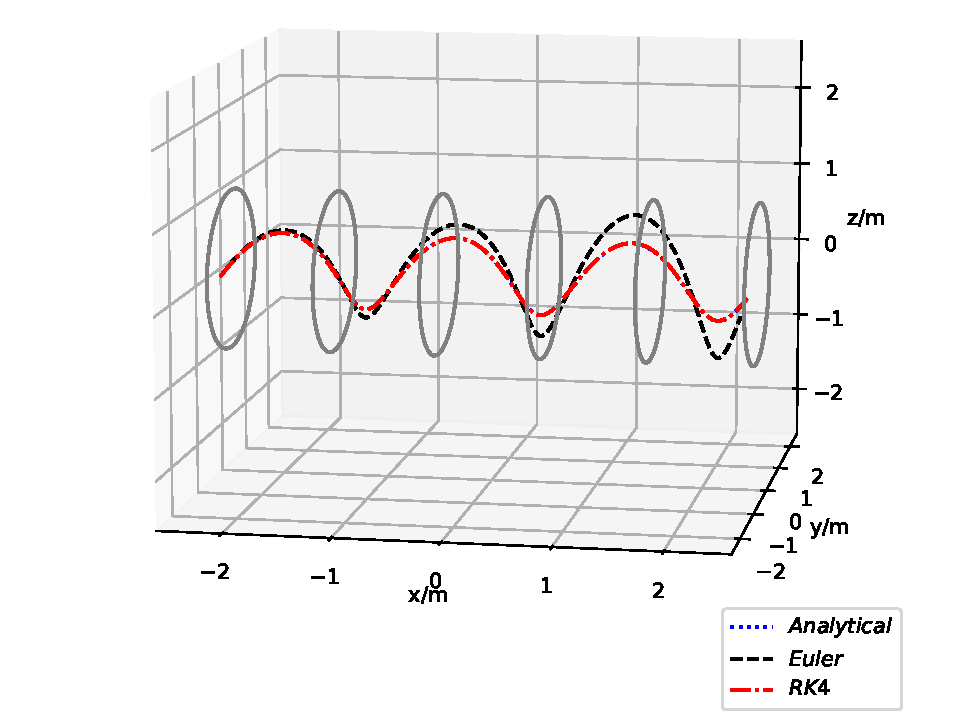
\includegraphics[height=0.9\beamer@frametextheight]{Solenoid_compare01_3D.pdf}

            312 steps
        }
    }
\end{frame}
\makeatother

\makeatletter
\begin{frame}
\frametitle{At a glance, 3D view.}
    \global\beamer@shrinktrue
    \gdef\beamer@shrinkframebox{
        \setbox\beamer@framebox=\vbox to\beamer@frametextheight{
            \centering
            $\Delta t_{equiv}\approx 1/10 T_c$

            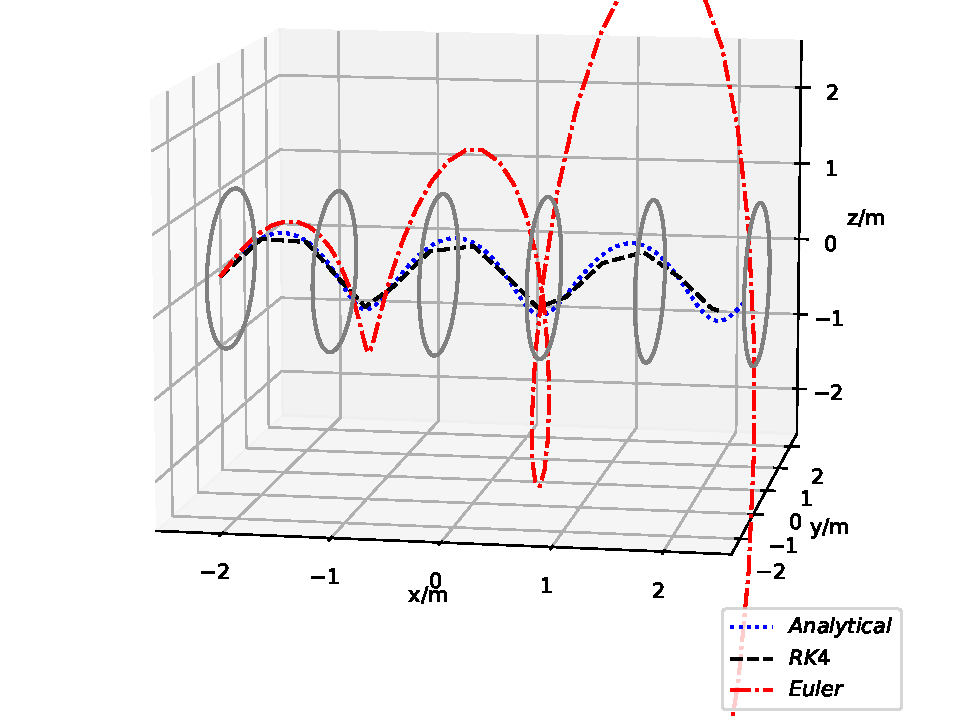
\includegraphics[height=0.9\beamer@frametextheight]{Solenoid_compare1_3D.pdf}

            31 steps.
        }
    }
\end{frame}
\makeatother

\begin{frame}
\frametitle{At a glance, front view, no border.}
\only<1>{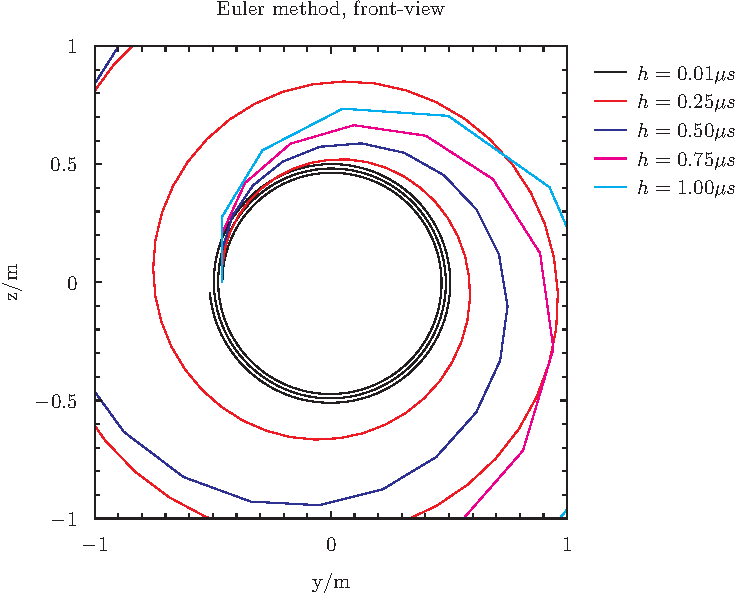
\includegraphics[width=\linewidth]{solenoid_euler_yz_view.pdf}}%
\only<2>{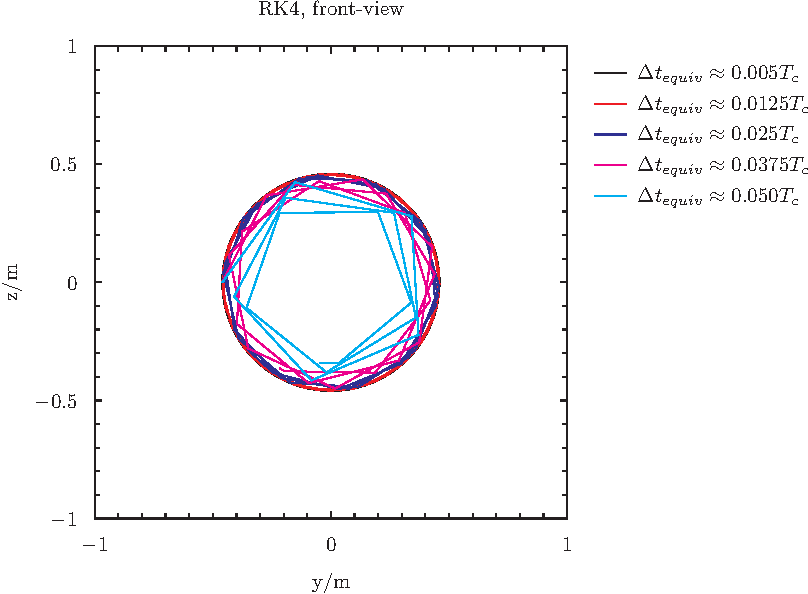
\includegraphics[width=\linewidth]{solenoid_RK_yz_view.pdf}}
\end{frame}

\begin{frame}
\frametitle{Error as function of $\Delta t_{equiv}$.}
\only<1>{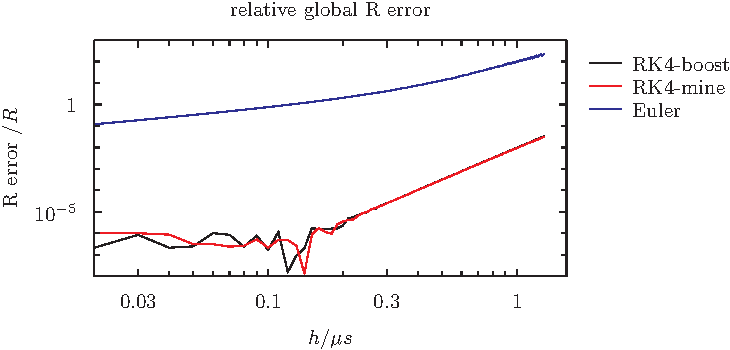
\includegraphics[width=\linewidth]{solenoid_Rh.pdf}}%
\end{frame}


\ifdraft
    \section{Embedded algorithms, and adaptive step size 15 min}
\else
    \section{Embedded algorithms, and adaptive step size}
\fi


\begin{frame}
\frametitle{What is not to like?}

\begin{columns}
\begin{column}{0.5\linewidth}
\begin{itemize}
\item <2-> Usually don't know error.

\item <2-> Hard to pick $\Delta t$ , and may change:

\item <3-> Inhomogeneous or time dependent fields (here, a true dipole).

\item <4-> Let the computer pick $\Delta t$ for error.

\end{itemize}
\end{column}
\begin{column}{0.5\linewidth}

\only<3->{
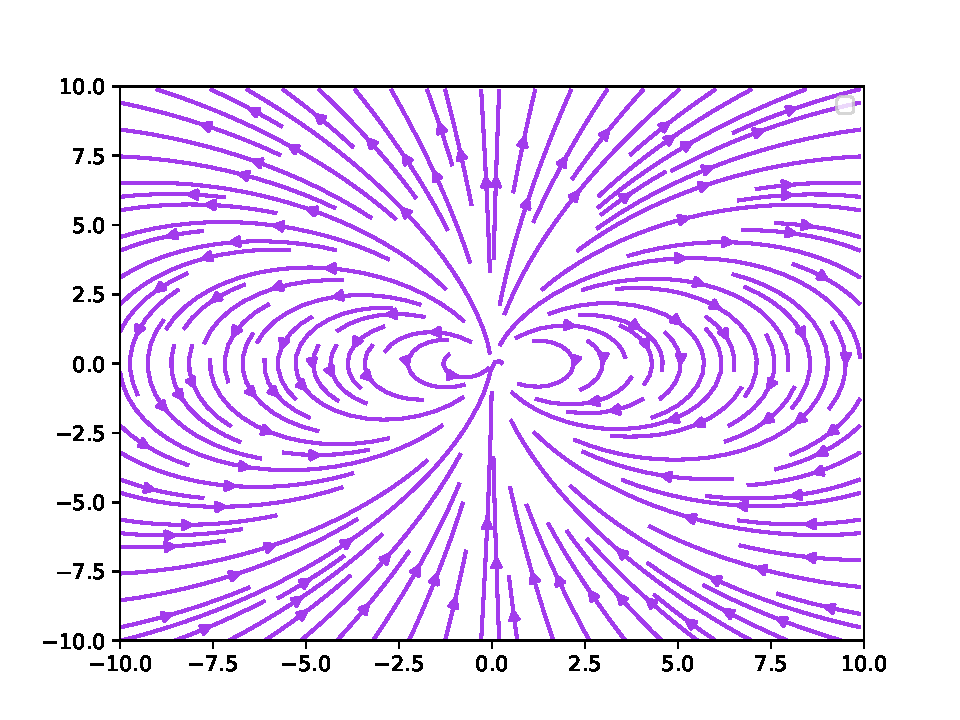
\includegraphics[width=\linewidth]{dipole.pdf}
}
\end{column}
\end{columns}
\end{frame}



\subsection{Dormand Prince 5 (4) method}

\begin{frame}
\frametitle{Embedded Runge-Kutta algorithms.}
\begin{itemize}
\item <1-> Need estimate for error.

\item <2-> Runge-Kutta step $\mathbf{X}^{(p)}(t_{i+1})$ will converge to $\mathbf{X}(t_{i+1})$.
\item <3-> Use 2 different order methods, $\mathbf{X}^{(p-1)}(t_{i+1})$, $\mathbf{X}^{(p)}(t_{i+1})$.

\item <4-> Approximate ``Error" as  $\mathbf{E}_j = |\mathbf{X}^{(p-1)}_j(t_{i+1})-\mathbf{X}^{(p)}_j(t_{i+1})|$.

\item <5-> Adjust step size to keep the error(s) small (Implementations differ!).

{\color{gray} Dormand, J. R.; Prince, P. J. (1980), "A family of embedded Runge-Kutta formulae", Journal of Computational and AppliMathematics.}
\end{itemize}
\end{frame}


\begin{frame}
\frametitle{Runge-Kutta Dormand Prince 5 (4).}

\begin{itemize}
\item <1->\lstinline{ode45} in Matlab, \lstinline{scipy.solve_ivp} in Python , \lstinline{RungeKutta_dopri5} in \lstinline{boost::odeint}.

\begin{align*}
\mathbf{X}^{(5)}(t_{i+1})-\mathbf{X}(t_{i}) &=  \Delta t \sum_{j=1}^{m} b_j^{(5)} \mathbf{K}_j\\
\mathbf{X}^{(4)}(t_{i+1})-\mathbf{X}(t_{i}) &=  \Delta t \sum_{j=1}^{m} b_j^{(4)} \mathbf{K}_j.
\end{align*}

\begin{align*}
\mathbf{K}_j &= \mathbf{f}_{ode}(\mathbf{X}(t_i)+\Delta t \sum_k^{j-1} a_{kj} \mathbf{K}_j,t_i+c_3 \Delta t).
\end{align*}

\item <2-> 7 $\mathbf{K}_j$'s (actually 6 by clever re-usage) (First same as last principle).

{\color{gray} Dormand, J. R.; Prince, P. J. (1980), "A family of embedded Runge-Kutta formulae", Journal of Computational and Applied Mathematics}
\end{itemize}
\end{frame}

\begin{frame}
\frametitle{Butcher Tableu of Dormand Prince (5) 4.}

{\renewcommand{\arraystretch}{1.2}
\begin{tabular}{c | @{\quad} c @{\quad} c @{\quad} c @{\quad} c @{\quad} c @{\quad} c @{\quad} c @{\quad} c}
$c_i$ & $a_{ij}$ & $\hdots$\\
\midrule
$0$ \\
$\frac{1}{5}$ & $\frac{1}{5}$\\
$\frac{3}{10}$ & $\frac{3}{40}$ &  $\frac{9}{40}$\\
$\frac{4}{5}$ & $\frac{40}{45}$ &  $-\frac{56}{15}$  &  $-\frac{32}{9}$\\
$\frac{8}{9}$ & $\frac{19372}{6561}$ & $-\frac{25360}{2187}$ & $\frac{64448}{6561}$ & $-\frac{212}{729}$\\
$1$ & $\frac{9017}{3168}$ & $-\frac{355}{33}$ & $\frac{46732}{5247}$ & $\frac{49}{176}$  & $-\frac{5103}{18656}$\\
$1$ & $\frac{35}{384}$  & $0$	 & $\frac{500}{1113}$ & $\frac{125}{192}$ & $-\frac{2187}{6784}$ & $\frac{11}{84}$\\
\midrule
$/b^{(5)}$  & $\frac{35}{384}$ & $0$ & $\frac{500}{1113}$ & $\frac{125}{192}$ & $-\frac{2187}{6784}$ & $\frac{11}{84}$ & $0$\\
$/b^{(4)}$ & $\frac{5179}{57600}$ & $0$ & $\frac{7571}{16695}$ & & $\frac{393}{640}$ & $-\frac{92097}{339200}$& $\frac{187}{2100}$ & $\frac{1}{40}$
\end{tabular}
}
\end{frame}

\begin{frame}
\frametitle{Runge-Kutta Dormand Prince 5 (4).}

\begin{itemize}
\item <1-> Adaptive step size (Dormand Prince):

\begin{align*}
 \Delta t_{new}  = 0.9  \Delta t_{old}  \left[\frac{\delta }{||\mathrm{E}||}\right]^{\frac{1}{p+1}}
\end{align*}

\item <2-> Adaptive step size (My version):

\begin{align*}
 \Delta t_{new}  &= \min_j \left(0.9  \Delta t_{old}  \left[\frac{\delta_j}{\mathrm{E}_{j}}\right]^{\frac{1}{p}}\right), \quad \mathrm{E}_j>\delta_j : \mathrm{reject}\\
\delta_j &=\min(\delta_{abs},|\mathbf{X}_j(t_{i})|\delta_{rel})\sqrt{\frac{ \Delta t_{old} }{T}}.
\end{align*}

\item <3-> Scale by step size $\frac{ \Delta t_{old} }{T}$, ``Fail safe" $\sqrt{\ldots}$.

{\color{gray} Dormand, J. R.; Prince, P. J. (1980), "A family of embedded Runge-Kutta formulae", Journal of Computational and Applied Mathematics.}
\end{itemize}
\end{frame}

\subsection{Demonstration: magnetic dipole}

\begin{frame}
\frametitle{Does it work?}
\begin{centering}
\only<1>{%
\noindent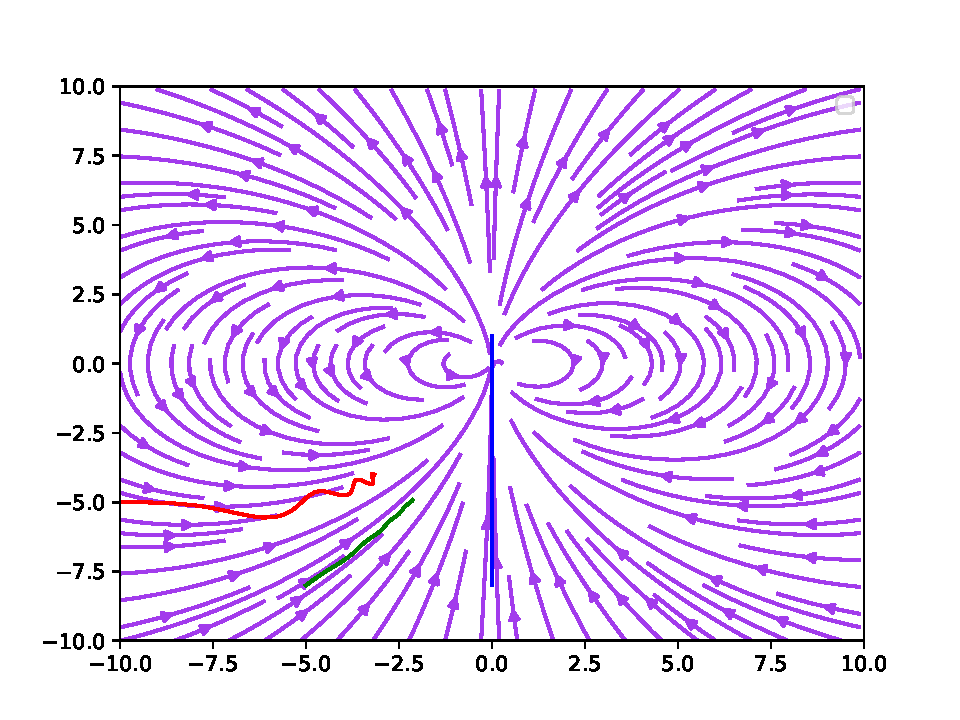
\includegraphics[width=0.8\linewidth]{dipole2.pdf}

My version relative and absolute error $10^{-6}$. 313 steps (+ 25 rejected).

}%
\only<2>{%
\noindent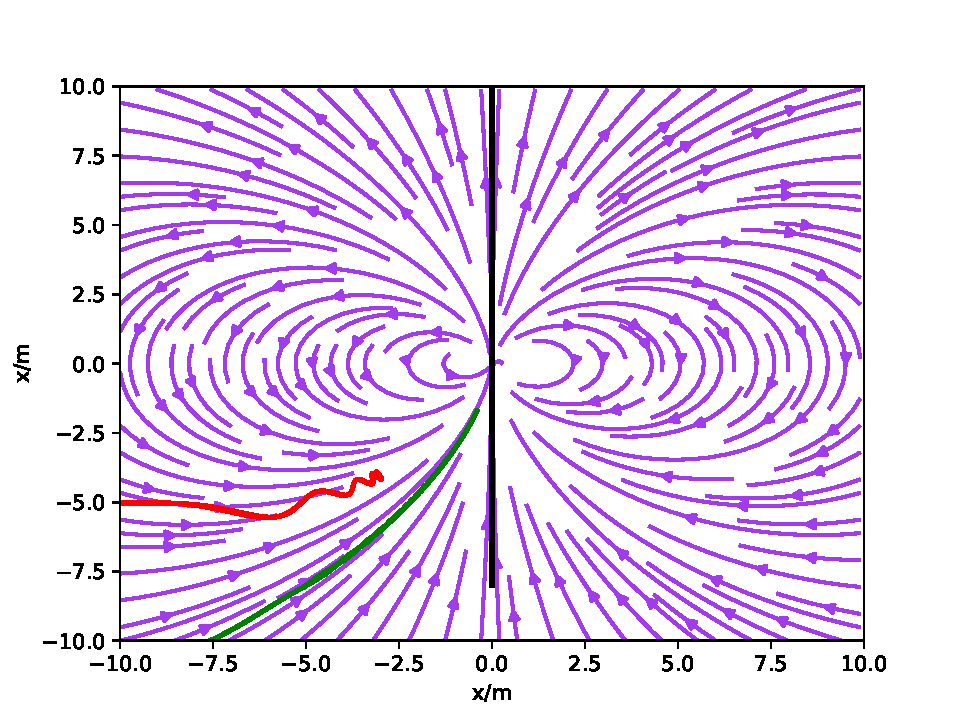
\includegraphics[width=0.8\linewidth]{dipole3.pdf}

Odeint library relative and absolute error $10^{-7}$. 249 steps.
}%
\only<3>{%
\noindent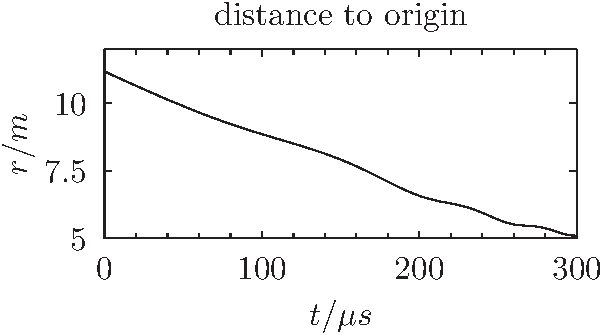
\includegraphics[width=\linewidth]{dipole_R.pdf}}%
\only<4>{%
\noindent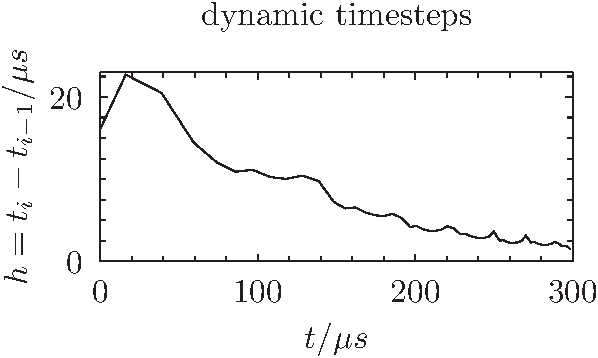
\includegraphics[width=\linewidth]{dipole_h.pdf}

My version, adaptive step size.
}%



\end{centering}
\end{frame}



\section{Conclusion}

\begin{frame}
\frametitle{Conclusion.}
\begin{itemize}
\item<1-> Simulating particles in electric and magnetic fields.
\item<2-> Numerically solving ordinary differential equations.
\item<2-> Can easily be generalized to other systems.
\end{itemize}
\end{frame}

%\subsection{If time permits, the cyclotron}

\begin{frame}
\frametitle{Example, cyclotron.}
\begin{columns}
\begin{column}{0.5\linewidth}
\begin{itemize}
\item<1-> Electric field accelerates, magnetic contains.

\item<2-> Single gab, oscillating field.

\item<3-> Uses classical Cyclotron frequency.

\item<4-> Analytical final speed, in principle path.

\begin{equation*}
\frac{R|q|B}{m} = v_\perp.
\end{equation*}

\end{itemize}
\end{column}
\begin{column}{0.5\linewidth}
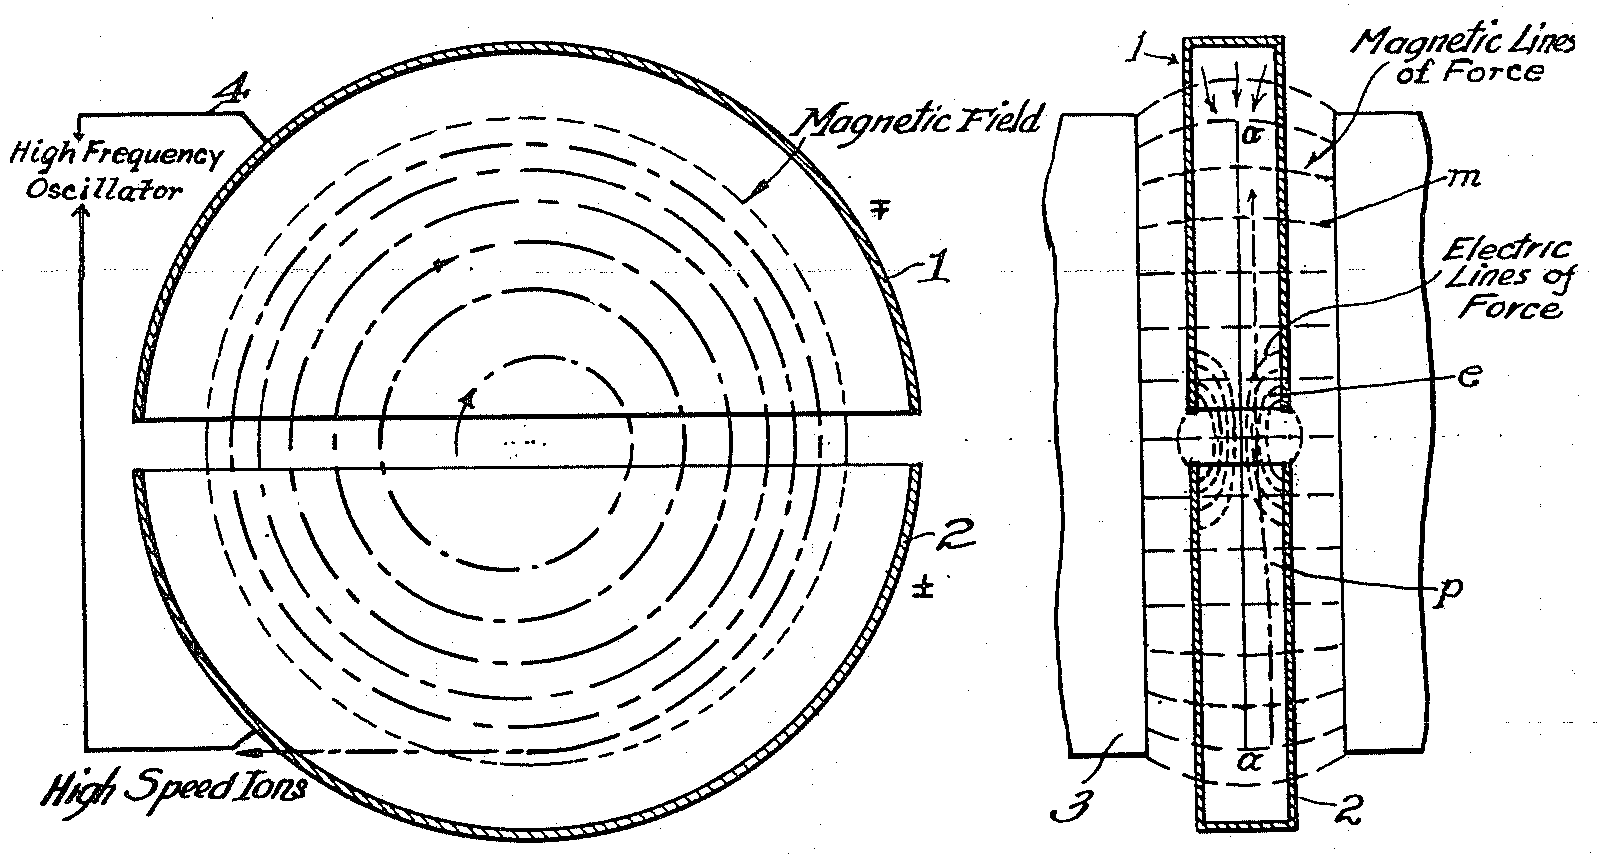
\includegraphics[width=\linewidth]{ Cyclotron_patent.png}
{\color{gray} Ernest O. Lawrence, 1934, U.S. Patent 1,948,384; image in Public Domain.}
\end{column}
\end{columns}
\end{frame}



\begin{frame}
\frametitle{can it be simulated.}
\begin{columns}
\begin{column}{0.5\linewidth}
\begin{itemize}
\item<1-> with fixed step size, looks bad 4999 points.

\item<2- > my adabtive method, error: $10^{-6}$.

\item<2- > Looks great but 2 million points.

\item<3-> odeint library.

\item<4-> non-continuous ode are bad.

\end{itemize}
\end{column}
\begin{column}{0.5\linewidth}
\only<1>{%
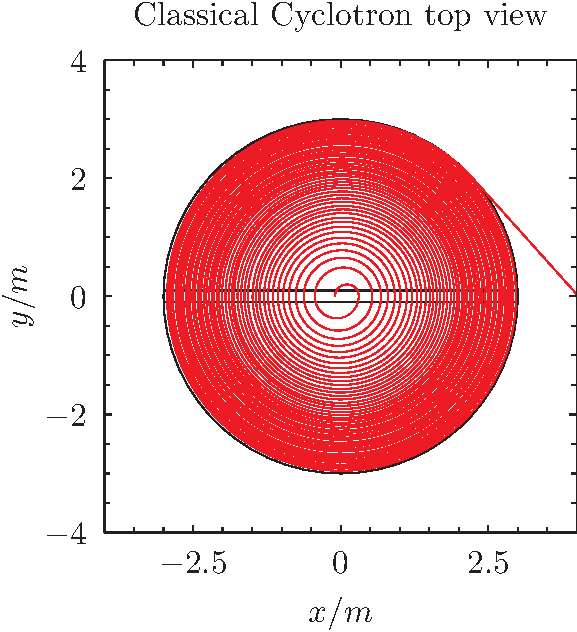
\includegraphics[width=\linewidth]{ cyclotron_noadapt_xy-view.pdf}%

}%
\only<2>{%
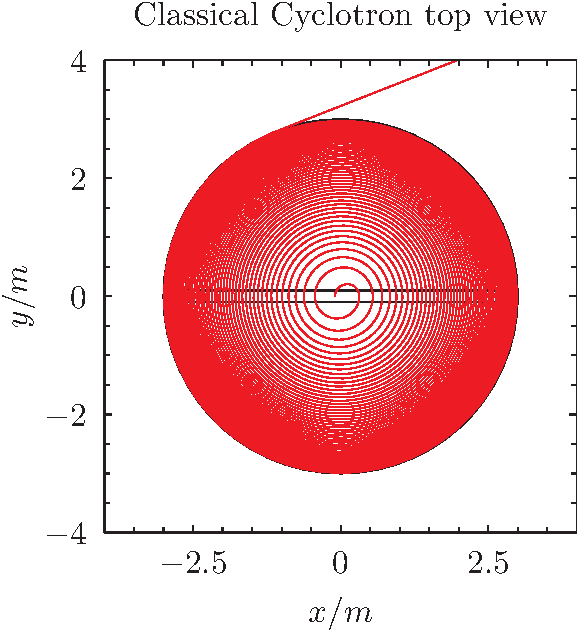
\includegraphics[width=\linewidth]{ cyclotron_overadapt_xy-view.pdf}%

}%
\only<3->{%
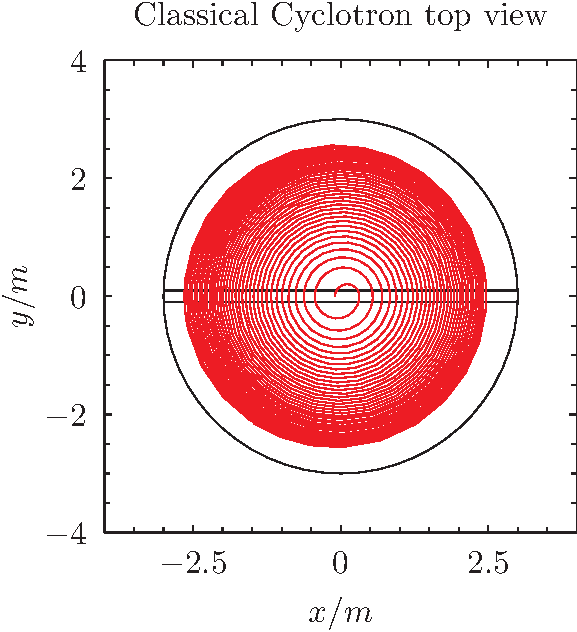
\includegraphics[width=\linewidth]{ cyclotron_badadapt_xy-view.pdf}%
}%

\end{column}
\end{columns}
\end{frame}


%\subsection{If time permits, Cycloid motion.}
%\subsection{If time permits, Toroidal coils.}

\end{document}
